\subsection{Elektrotechnik}

\subsubsection{Übersicht}
Die Elektronik ist organisiert in einem modularen Verbund von verschiedenen
Funktionsgruppen. Nebst den elementaren Einheiten wie Motoren und zugehörigen
Treibern gehören auch etwa Pegelwandler und Sensoren dazu. Die Abbildung
\ref{fig:et-block} zeigt schematisch den Zusammenhang dieser Komponenten.


\begin{figure}[h!]
	\centering	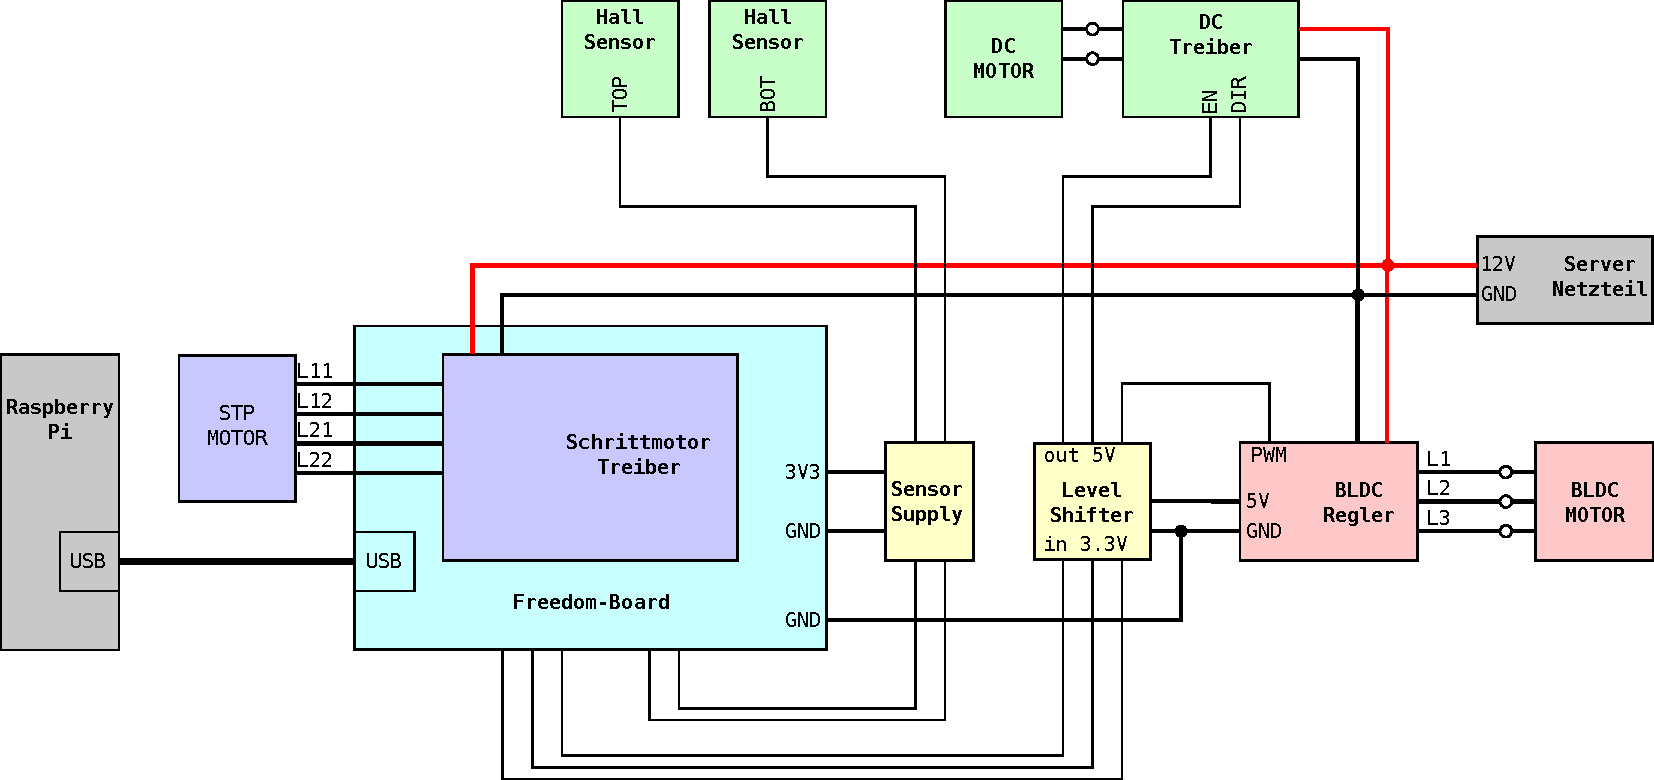
\includegraphics[width=0.95\textwidth]{../../fig/blockdiagram.pdf}
	\caption{Blockschaltbild der Elektrokomponenten}
	\label{fig:et-block}
\end{figure}
	% Übersicht
\newpage
\subsubsection{Speisung}

Die Speisung ist mehrstufig realisiert. Zum einen gibt es eine Speisung
welche die Energie für die Logikeinheiten liefert. Diese wird per Netzadapter
an das Raspberry Pi geführt. Dieses bildet die High-Level-Logik und somit die
zentrale Einheit welche eine 5 Volt Speisung zur Verfügung stellt an den
USB-Schnittstellen des Einplatinencomputers. Das Raspberry Pi wird per
USB-Kabel mit dem Freedomboard verbunden, über welches nebst den
Datenleitungen auch die Speisung geführt wird. So ist sichergestellt,
dass beide Einheiten eine gemeinsame Speisung haben welche auch der
logischen Hierarchie folgt. Das Freedomboard selbst stellt eine weitere
Speisung bereit auf dem eigenen Logikpegel von 3.3 Volt. Die Abbildung
\ref{fig:et-block_logic} zeigt das Blockschaltbild mit ausgeblendeten
Einheiten welche nicht von der Logikspeisung betrieben werden.

\begin{figure}[h!]
	\centering
	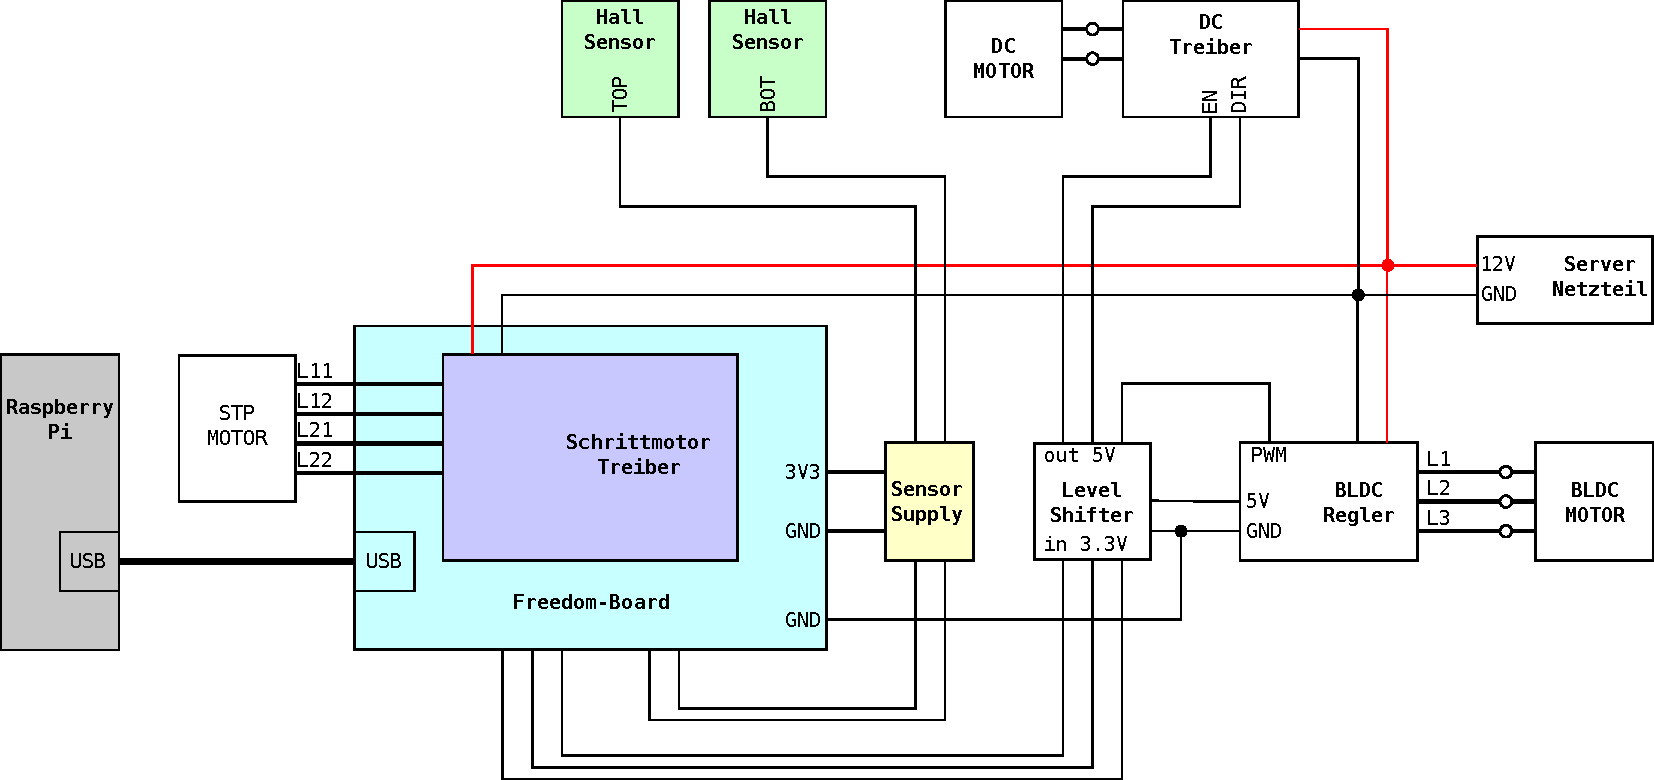
\includegraphics[width=0.95\textwidth]{../../fig/blockdiagram_logic.pdf}
	\caption{Blockschaltbild der Logikspeisung}
	\label{fig:et-block_logic}
\end{figure}

Nebst der Speisung für die Logik, welche auch die Kommunikation zwischen
Raspberry Pi und Freedomboard ermöglicht, bedarf es auch einer
Leistungsspeisung. Diese wird mittels eines Servernetzteils zur Verfügung
gestellt. Das Servernetzteil bietet eine 12 Volt Speisung welche für sämtliche
Motoren eingesetzt wird. Auf diese Weise kann eine satte Speisung
gewährleistet werden welche auch für höhere Leistungsänderungen fähig ist.
Nebst den Motoren und den zugehörigen Treibern wird auch der 3.3 Volt zu 
5 Volt Pegelwandler durch die Leistungsspeisung betrieben. Hierzu wird der
interne 5 Volt Spannungsregler der Brushlessansteuerung genutzt, welcher durch
die Leistungsspeisung betrieben wird. Dies garantiert stabile Pegel für die
Ansteuerung des Brushlessreglers so wie dies im beabsichtigen Einsatz
vorgesehen ist.



	% Speisung
\newpage
\subsubsection{BLDC-Motor}
Der Antrieb für den Ballabwurf ist realisiert mittels eines
Brushless-Gleichstrommotors vom Modell A20-12XL EVO von Hacker.
Dieser wird mittels eines passenden kommerziellen Reglers vom
Typ X-30 PRO betrieben. Der Regler wird gestellt durch die Firmware
des Freedomboards, welche per UART bedient wird.

Die zugehörige Software kann mittels des UART-Interfaces per
Kommandozeile bedient werden mit dem Befehl \verb!BLDC! und den
zugehörigen Parametern. Die komplette Liste aller Befehle zu
\verb!BLDC! kann mittels \verb!BLDC help! aufgerufen werden.

\begin{figure}[h!]
	\centering
	\begin{subfigure}[b]{0.45\textwidth}
		\centering
		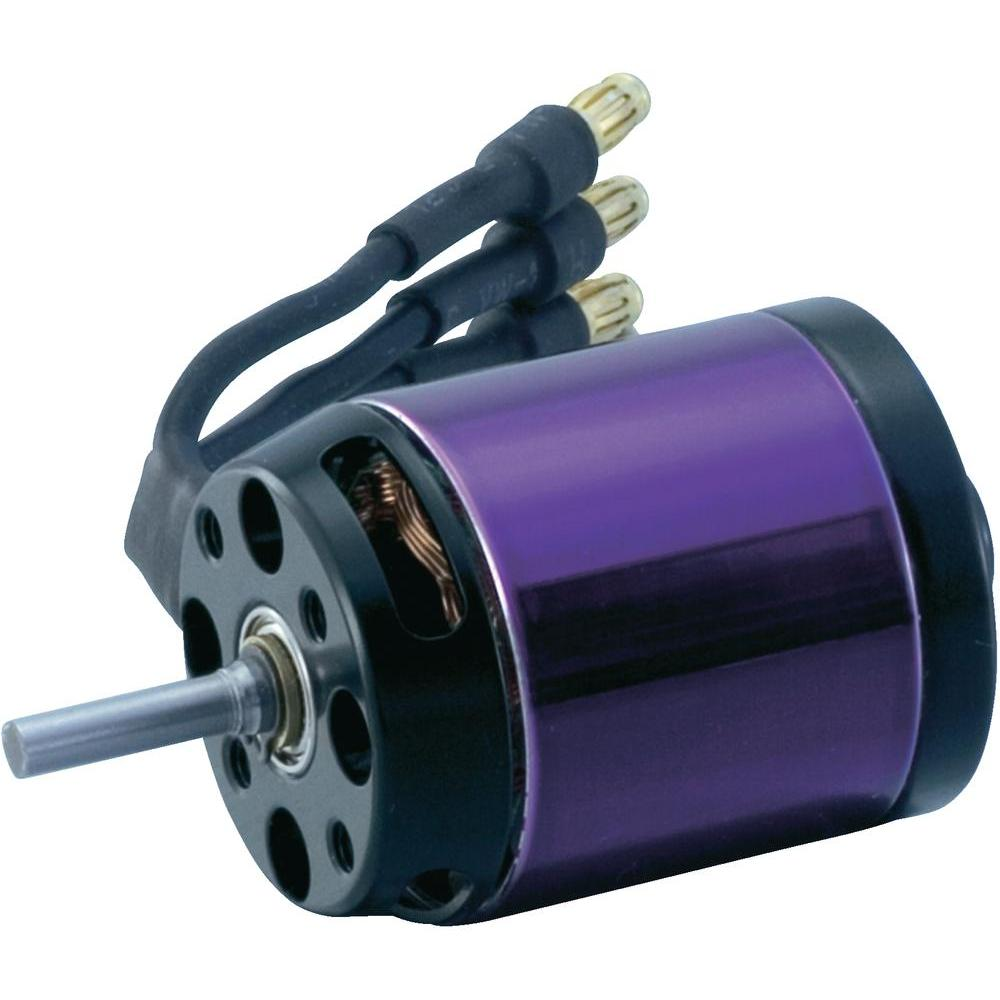
\includegraphics[width=0.75\textwidth]{../../fig/et/a20_12xl_evo.jpg}
		\caption{BLDC-Motor Hacker A20-12XL EVO}
	\end{subfigure}
	\begin{subfigure}[b]{0.45\textwidth}
		\centering
		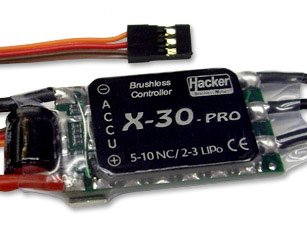
\includegraphics[width=0.75\textwidth]{../../fig/et/x30_pro.jpg}
		\caption{BLDC-Motor Hacker X-30 PRO}
	\end{subfigure}
	\caption{Antriebssystem für den Ballabwurf}
\end{figure}

Da ein kommerzieller Regler verwendet wird aus dem Modellbau für
Flugzeuge und Helikopter, kann lediglich ein Standard PWM-Signal
aus dem Modellbau benutzt werden, um die Drehzahl des Motors zu
stellen. Da dieser Regler eine echte Drehzahlregelung implementiert
wird auf einen überlagerten Regler auf dem Freedomboard verzichtet.
Eine allfällige Parametierung kann mittels eines Programmieradapters
X-PRO USB Controller V2 des Herstellers vorgenommen werden.
		% BLDC Motor / Ballabwurf
\newpage
\subsubsection{DC-Motor}
Der DC-Motor dient dem Vorschub der Bälle. Diese werden so dem
Abwurfmechanismus zugeführt, welche dieser dann selbstständig
greift und mittels des Schwungrades abwirft. Hierzu wird ein
einfacher und kräftiger Bürstenmotor verwendet vom Typ Xdrive
555-1 der Marke Motraxx.

\begin{figure}[h!]
	\centering
	\begin{subfigure}[b]{0.45\textwidth}
		\centering
		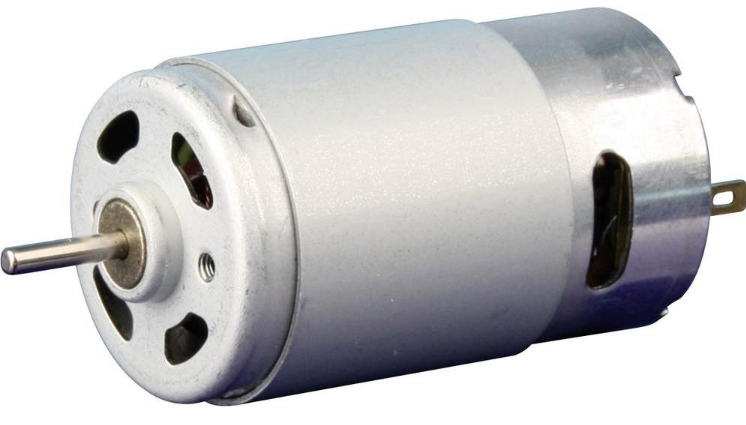
\includegraphics[width=1\textwidth]{../../fig/et/dc_01.png}
		\caption{Gleichstrommotor Xdrive 555-1 von Motraxx}
	\end{subfigure}
	\begin{subfigure}[b]{0.45\textwidth}
		\centering
		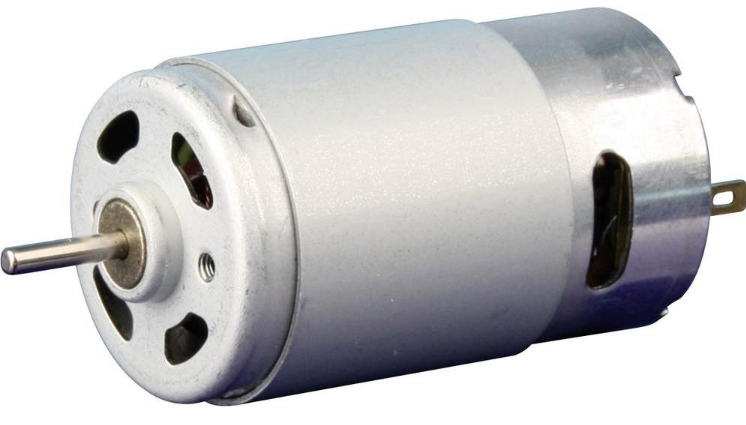
\includegraphics[width=1\textwidth]{../../fig/et/dc_01.png}
		\caption{DC-Treiberboard der Gruppe PREN-ET}
	\end{subfigure}
	\caption{Motor und Elektronik des Ballvorschubs}
\end{figure}

Für die Ansteuerung des DC-Motors wird ein eigens in der Gruppe
PREN-ET entwickeltes Board verwendet. Dieses beinhaltet als
Kernelement den Treiberchip A3941 von Maxim. Dieser bietet die
Möglichkeit das PWM Signal einzuspielen und so die gemittelte
Motorspannung zu stellen. Diese wird mittels einer
MOSFET-Vollbrücke über dem Motor eingestellt. Für die vorliegende
Implementierung ist dabei die externe PWM Vorgabe deaktiviert.
Dieses wird on-board erzeugt und ist mittels eines
Trimmpotentiometers eingestellt. Das so konfigurierte Board
bietet nun ein einfaches Interface welches lediglich zwei
Eingangssignale kennt: Enable (Ein / Aus) und Direction (Aufwärts
/ Abwärts).
%
%\begin{itemize}
%	\item Enable \hfill{Ein / Aus}
%	\item Direction \hfill{Aufwärts / Abwärts}
%\end{itemize}
%
Die vollständige Dokumentation des Treiberboards ist auf dem
Gruppenrepository \url{https://github.com/pren-et/doc}
von PREN-ET zu finden oder im Anhang \ref{sec:dc_doc} einsehbar.
Die Bedienung des Treiberboards ist vollständig in der Firmware des
Freedomboards implementiert und in der Shell verfügbar. Hierzu kann
das Kommando \verb!DC! verwendet werden.

Eine gekoppelte Komponente stellen jeweils die Endschalter dar.
Diese sind fester Bestandteil der Ansteuerungsfirmware des
Treiberboards und implementiert einige Automatismen zum Schutz
des Motors und zum einwandfreien einsatz des Ballvorschubs.
		% DC Motor / Ballnachschub
\newpage
\subsubsection{Schrittmotor}
Der Schrittmotor dient der horizontalen Ausrichtung des Maschinenturms.
Hierzu ist der Schrittmotor fix eingebaut im Turm und greift per Zahnrad
in einen Kranz der Bodenplatte. Mit dem Drehen des Zahnrades rotiert der
Turm zur entsprechenden Seite. Hierfür ist ein Schrittmotor vom Typ 
QSH4218-51-10-049 von Trinamic.

\begin{figure}[h!]
	\centering
	\begin{subfigure}[b]{0.45\textwidth}
		\centering
		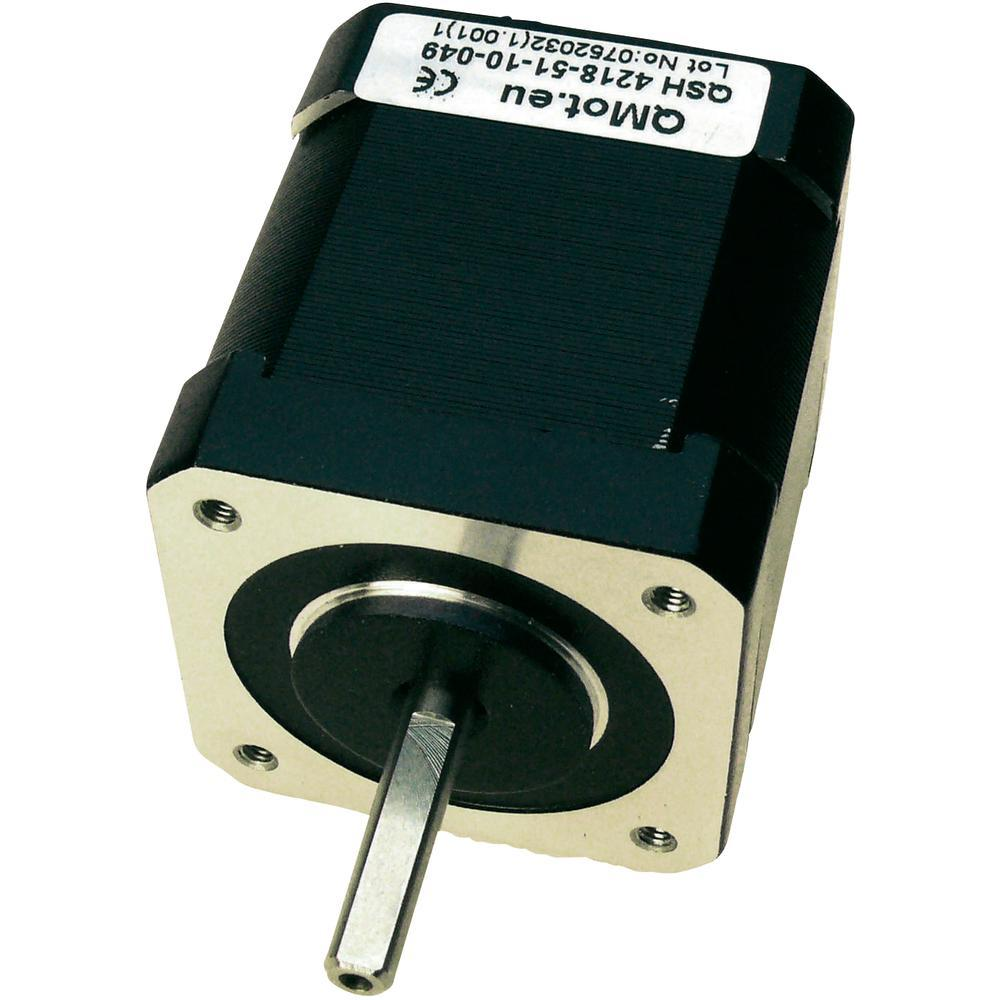
\includegraphics[width=1\textwidth]{../../fig/et/QSH4218-51-10-049.jpg}
		\caption{Schrittmotor QSH4218-51-10-049}
	\end{subfigure}
	\begin{subfigure}[b]{0.45\textwidth}
		\centering
		\includegraphics[width=1\textwidth]{../../fig/et/stepper_pcb.png}
		\caption{Stepper-Treiberboard von PREN-ET}
	\end{subfigure}
	\caption{Motor und Elektronik des Schrittmotors}
\end{figure}

Für die Ansteuerung des Schrittmotors ist ein von der Gruppe PREN-ET
entwickeltes Shield für das Freedomboard im Einsatz. Dieses beinhaltet
als Kernkomponente den Treiberchip L6480 von ST Microelectronics. Dieser
implementiert sämtliche Funktionalitäten und Ansteuerungsverfahren für den
Schrittmotor inklusive Optimierungsmöglichkeiten. Der Chip wird dabei
mittels einer SPI Verbindung von Freedomboard aus gesteuert.
	% Schrittmotor / Ausrichtung
\newpage
\subsubsection{Endschalter}
Für den Ballvorschub sind elektronische und kontaktlose Endschalter
eingesetzt, welche das Erreichen der Endposition erkennen für den
Ballvorschub. Dies ist eine wichtige Schutzmassnahme, da diese
nicht in den Anschlag gehen darf, was den Motor des Vorschubs
überansprucht.

Für diese Funktion sind magnetisch getriggerte Hall-Effekt-Schalter
eingesetzt vom Typ AH180N von Diodes Incorporated. Hierzu sind eigens
etstellte Platinen der PREN-ET Subgruppe DC im Einsatz.

\begin{figure}[h!]
	\centering
	\begin{subfigure}[b]{0.45\textwidth}
		\centering
		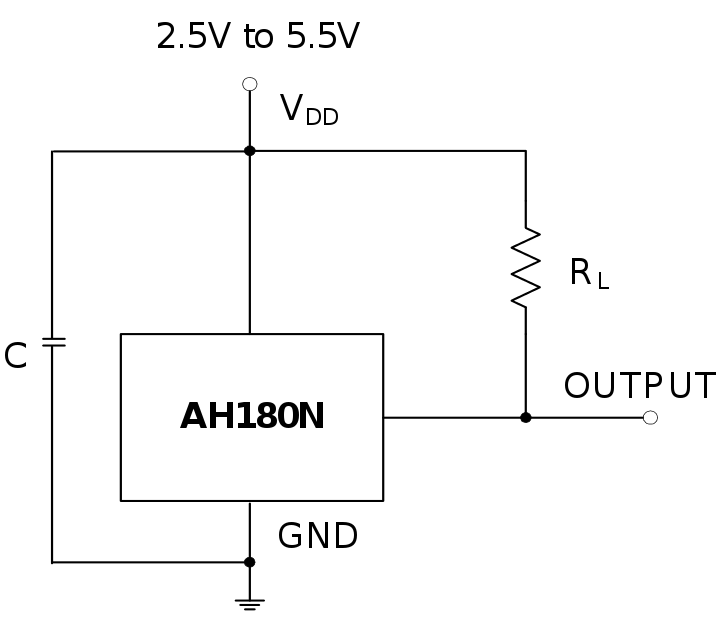
\includegraphics[width=1\textwidth]{../../fig/et/ah180n.png}
		\caption{Typical Application AH180N}
	\end{subfigure}
	\begin{subfigure}[b]{0.45\textwidth}
		\centering
		%\includegraphics[width=1\textwidth]{../../fig/et/}
		\caption{Endschalter-Platine}
	\end{subfigure}
	\caption{Endschalter für den Ballvorschub}
\end{figure}

Die Hall-Effekt-Schalter werden mit der vom Freedomboard zur Verfügung
gestellten 3.3 Volt Speisung betrieben. Da die Ausgangsstufe des Sensors
als Open-Collector implementiert ist, kann so das 3.3 Volt Signal direkt
auf das Freedomboard zurückgeführt und verarbeitet werden. 

Die Signale der Endschalter sind als Interruptquellen in der Firmware des
Freedomboard implementiert und reagieren auf fallende Signalflanken. Da
der Hall-Effekt-Schalter eine Hysterese besitzt, gibt es ein sauberes
Signal an den Eingängen ohne Prellen.

Die Firmware bindet die Interrupts direkt an den Ballvorschub in der Weise,
dass der Motor unverzüglich abgestellt wird und präventiv die Drehrichtung
geändert wird. Die Änderung der Drehrichtung richtet sich nach dem
aktivierten Sensor. So wird die Drehrichtung auf Abwärts gestellt
falls der obere Endschalter ausschlägt und umgekehrt beim unteren.

Die Zustände der Endschalter können über die Statusanzeige vom DC-Motor
eingesehen werden auf der Kommandozeile. Die Quittierung der Sensoren
erfolgt per Einschalten des DC-Motors.

Die Firmware auf dem Freedomboard bietet noch zwei Besonderheiten im
Zusammenhang mit den Endschaltern. Zum einen sind beide per Default nach
einem Reset als aktiv gesetzt und zum anderen wird ein ausgeschlagener
Endschalter den Zustand der RGB-LED auf dem Freedomboard orange färben,
sonst ist diese grün.
	% Endschalter
%\input{content/et/nachschub}
%\input{content/et/ausrichtung}

% \subsubsection{Übersicht}
% Die Elektronik ist organisiert in einem modularen Verbund von verschiedenen
% Funktionsgruppen. Nebst den elementaren Einheiten wie Motoren und zugehörigen
% Treibern gehören auch etwa Pegelwandler und Sensoren dazu. Die Abbildung
% \ref{fig:et-block} zeigt schematisch den Zusammenhang dieser Komponenten.
% 
% 
% \begin{figure}[h!]
% 	\centering
% 	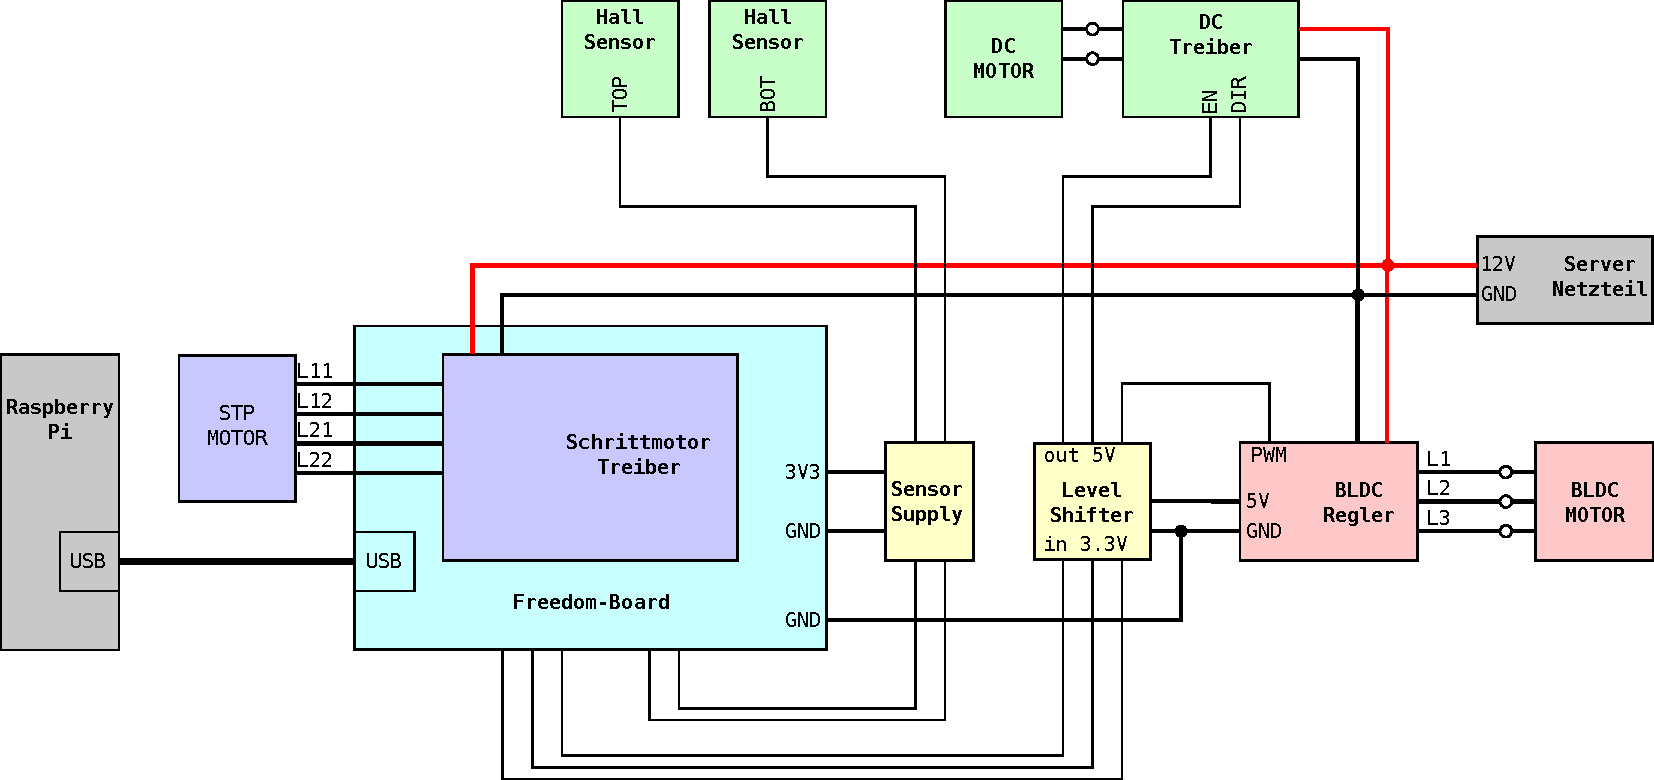
\includegraphics[width=0.95\textwidth]{../../fig/blockdiagram.pdf}
% 	\caption{Blockschaltbild der Elektrokomponenten}
% 	\label{fig:et-block}
% \end{figure}
% 
% \newpage
% \subsubsection{Speisung}
% 
% Die Speisung ist mehrstufig realisiert. Zum einen gibt es eine Speisung
% welche die Energie für die Logikeinheiten liefert. Diese wird per Netzadapter
% an das Raspberry Pi geführt. Dieses bildet die High-Level-Logik und somit die
% zentrale Einheit welche eine 5 Volt Speisung zur Verfügung stellt an den
% USB-Schnittstellen des Einplatinencomputers. Das Raspberry Pi wird per
% USB-Kabel mit dem Freedomboard verbunden, über welches nebst den
% Datenleitungen auch die Speisung geführt wird. So ist sichergestellt,
% dass beide Einheiten eine gemeinsame Speisung haben welche auch der
% logischen Hirachie folgt. Das Freedomboard selbst stellt eine weitere
% Speisung bereit auf dem eigenen Logikpegel von 3.3 Volt. Die Abbildung
% \ref{fig:et-block_logic} zeigt das Blockschaltbild mit ausgeblendeten
% Einheiten wleche nicht von der Logikspeisung betrieben werden.
% 
% \begin{figure}[h!]
% 	\centering
% 	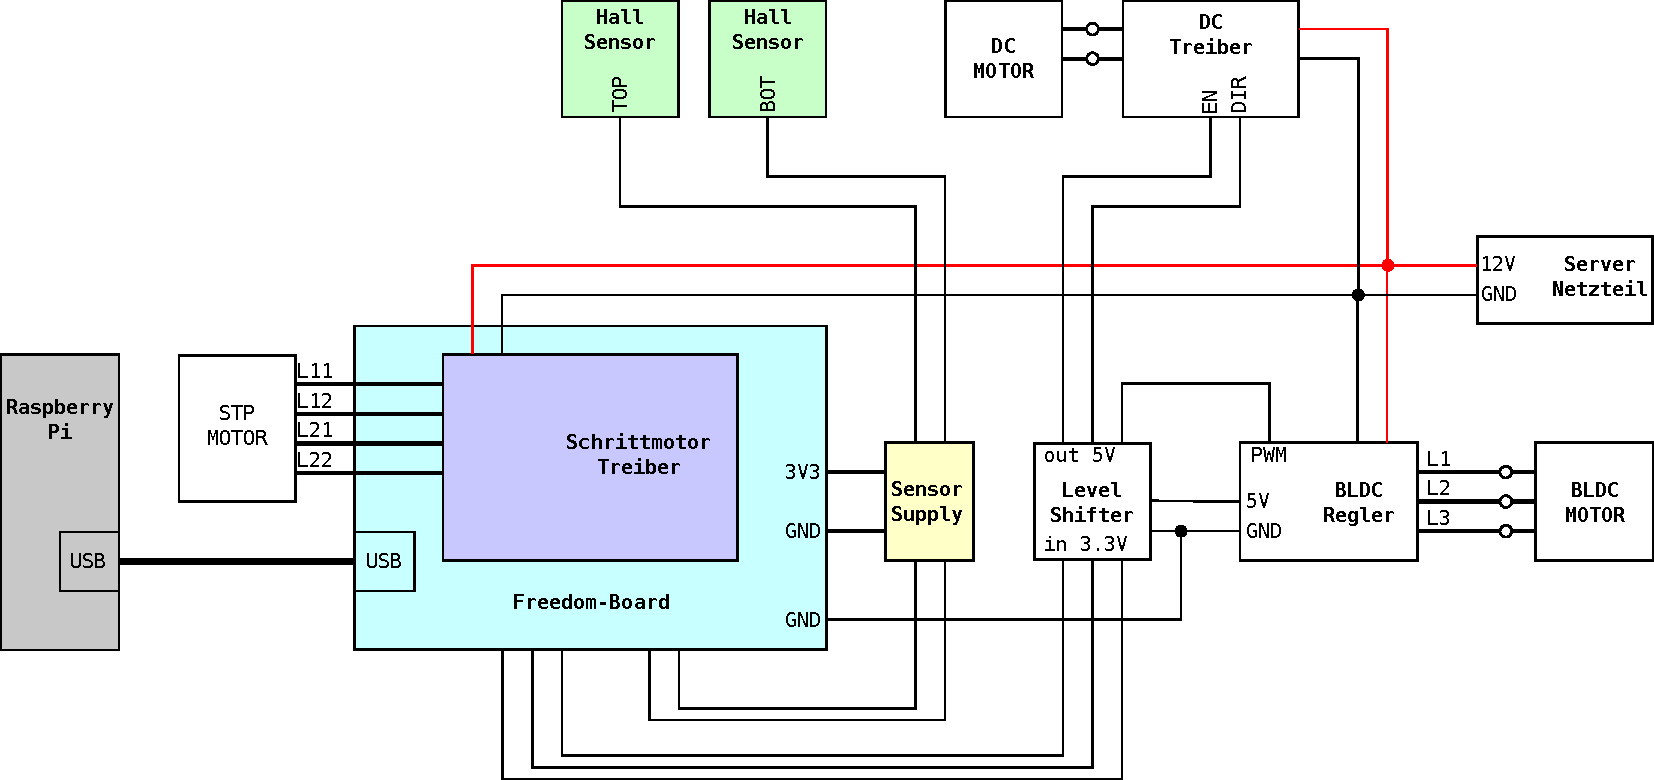
\includegraphics[width=0.95\textwidth]{../../fig/blockdiagram_logic.pdf}
% 	\caption{Blockschaltbild der Logikspeisung}
% 	\label{fig:et-block_logic}
% \end{figure}
% 
% Nebst der Speisung für die Logik, welche auch die Komminukation zwischen
% Raspberry Pi und Freedomboard ermöglicht, bedarf es auch einer
% Leistungsspeisung. Diese wird mittels eines Servernetzteils zur Verfügung
% gestellt. Das Servernetzteil bietet eine 12 Volt Speisung welche für sämtliche
% Motoren eingesetzt wird. Auf diese Weise kann eine satte Speisung
% gewährleistet werden wleche auch für höhere Leistungsänderungen fähig ist.
% Nebst den Motoren und den zugehörigen Treibern wird auch der 3.3 Volt zu 
% 5 Volt Pegelandler durch die Leistungsspeisung betrieben. Hierzu wird der
% interne 5 Volt Spannungsregler der Brushlessansteuerung genutzt, welcher durch
% die Leistungsspeisung betrieben wird. Dies garantiert stabile Pegel für die
% Ansteuerung des Brushlessreglers so wie dies im beabsichtigen Einsatz
% vorgesehen ist.



